\documentclass[11pt,border=0pt,tikz]{standalone}
\usepackage{csquotes}
\usepackage[backend=biber,style=numeric,sorting=none]{biblatex}

\providecommand{\FigScale}{1}

\usepackage{tikz}
\usetikzlibrary{decorations.pathmorphing, arrows.meta, calc, patterns}
\usepackage{amsmath}

\definecolor{coverbg}{rgb}{0,0.5333,0.2078}
\definecolor{seacol}{rgb}{0,0.42,0.16}
\definecolor{IBM5}{HTML}{ffb000}
\definecolor{IBM10}{HTML}{009e73}

\newcommand{\windturbine}{%
  \path[shade, left color=white, right color=gray!40, draw=gray!55, line width=0.4pt]
    (-0.55,0) -- (0.55,0) -- (0.18,6) -- (-0.18,6) -- (-0.55,0);
  \foreach \fy/\fw in {1.2/0.476, 3/0.365, 4.8/0.254} {
    \draw[gray!55, line width=0.4pt] (-\fw,\fy) -- (\fw,\fy);
  }
  \def\bladeScale{0.69}
  \foreach \ang in {30,150,270} {
    \begin{scope}[rotate around={\ang:(0,6.4)}]
      \begin{scope}[shift={(0,6.8)}, scale=\bladeScale, shift={(0,-6.8)}]
        \path[shade, top color=white, bottom color=gray!40, draw=gray!55, line width=0.4pt]
          (0.2,6.8)
          .. controls (0.65,7.51) and (0.45,9.00) .. (0.08,10.8)
          .. controls (0.0,11.04) and (-0.08,11.04) .. (-0.16,10.8)
          .. controls (-0.55,8.92) and (-0.75,7.35) .. (-0.2,6.8) -- (0.2,6.8);
      \end{scope}
    \end{scope}
  }
  \path[shade, left color=white, right color=gray!55, draw=gray!55] (0,6.4) circle (0.5);
}

\begin{document}
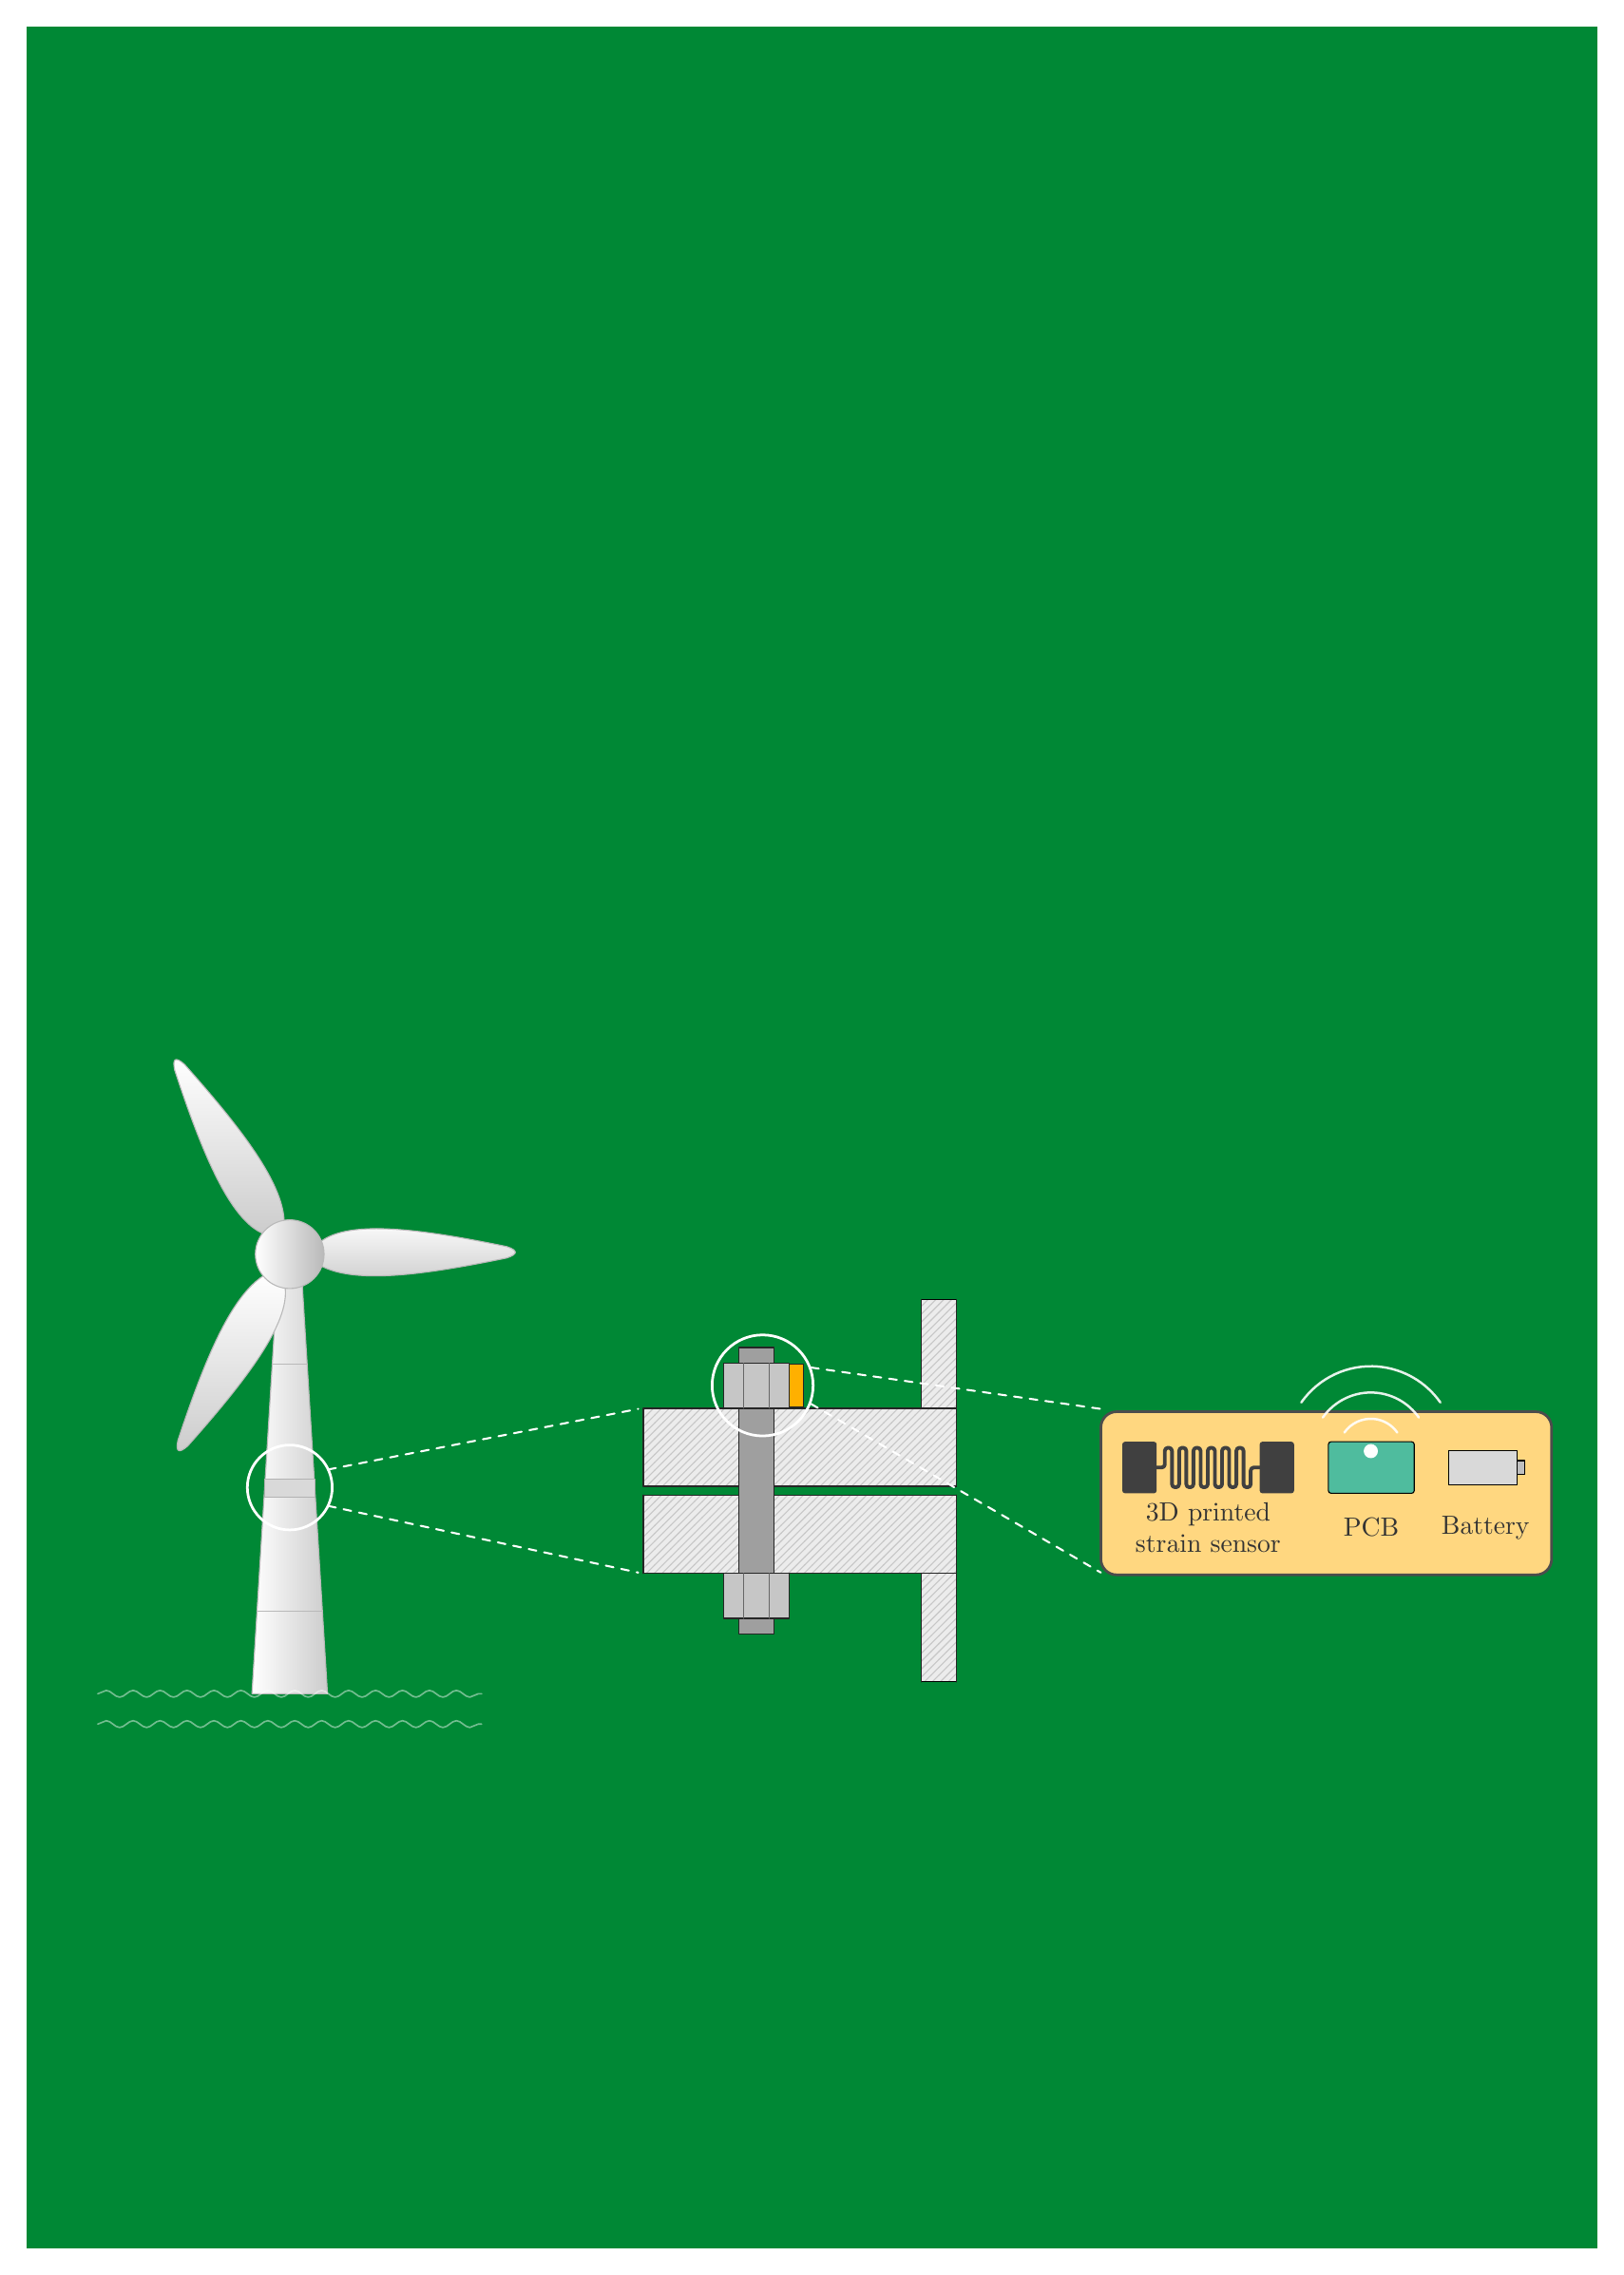
\begin{tikzpicture}[
  scale=\FigScale, line cap=round, line join=round,
  zoomline/.style={dashed, white, line width=0.75pt},
  zoomcirc/.style={white, line width=1.0pt},
  lbl/.style={font=\normalsize, text=black!80, align=center},
]

\fill[coverbg] (0,0) rectangle (21,29.7);
\path[use as bounding box] (0,0) rectangle (21,29.7);

\begin{scope}[shift={(10.5,11.6)}, scale=1.35, shift={(-8.57,-14.1)}]

% Turbine
\begin{scope}[shift={(3.4,11.0)}, scale=0.68]
  \windturbine
\end{scope}
\foreach \wy in {11.0,10.7} {
  \draw[white, line width=0.6pt, opacity=0.45, decorate,
        decoration={snake, amplitude=0.45mm, segment length=3.6mm}]
        (1.5,\wy) -- (5.3,\wy);
}
\coordinate (za) at (3.4,13.04);
\fill[gray!30, draw=gray!60, line width=0.3pt] (3.15,12.95) rectangle (3.65,13.13);
\draw[zoomcirc] (za) circle (0.42);
\draw[zoomline] (3.78,13.22) -- (6.85,13.82);
\draw[zoomline] (3.78,12.86) -- (6.85,12.2);

% Flange
\begin{scope}[shift={(2,10)}, scale=0.86]
  \fill[gray!15] (5.7,3.55) rectangle (9.3,4.45);
  \fill[gray!15] (8.9,4.45) rectangle (9.3,5.7);
  \fill[gray!15] (5.7,2.55) rectangle (9.3,3.45);
  \fill[gray!15] (8.9,1.3)  rectangle (9.3,2.55);
  \draw[pattern=north east lines, pattern color=black!22] (5.7,3.55) rectangle (9.3,4.45);
  \draw[pattern=north east lines, pattern color=black!22] (8.9,4.45) rectangle (9.3,5.7);
  \draw[pattern=north east lines, pattern color=black!22] (5.7,2.55) rectangle (9.3,3.45);
  \draw[pattern=north east lines, pattern color=black!22] (8.9,1.3) rectangle (9.3,2.55);
  \draw[black!85, line width=0.5pt]
       (5.7,4.45) -- (9.3,4.45) (5.7,3.55) -- (9.3,3.55)
       (5.7,3.45) -- (9.3,3.45) (5.7,2.55) -- (9.3,2.55)
       (5.7,3.55) -- (5.7,4.45) (5.7,2.55) -- (5.7,3.45)
       (9.3,2.55) -- (9.3,3.45) (9.3,3.55) -- (9.3,4.45);
  \draw[black!85, line width=0.5pt]
       (8.9,4.45) -- (8.9,5.7) (9.3,4.45) -- (9.3,5.7)
       (8.9,1.3) -- (8.9,2.55) (9.3,1.3) -- (9.3,2.55);
  \fill[gray!75, draw=black!85, line width=0.5pt] (6.8,1.85) rectangle (7.2,5.15);
  \fill[gray!45, draw=black!85, line width=0.5pt] (6.62,4.45) rectangle (7.38,4.97);
  \draw[black!60, line width=0.3pt] (6.85,4.45) -- (6.85,4.97) (7.15,4.45) -- (7.15,4.97);
  \fill[gray!45, draw=black!85, line width=0.5pt] (6.62,2.03) rectangle (7.38,2.55);
  \draw[black!60, line width=0.3pt] (6.85,2.03) -- (6.85,2.55) (7.15,2.03) -- (7.15,2.55);
  \fill[IBM5, draw=black!85, line width=0.4pt] (7.38,4.46) rectangle (7.54,4.96);
\end{scope}
\coordinate (zb) at (8.08,14.05);
\draw[zoomcirc] (zb) circle (0.5);
\draw[zoomline] (8.56,14.23) -- (11.43,13.82);
\draw[zoomline] (8.56,13.87) -- (11.43,12.2);

% Module
\begin{scope}[shift={(2.165,8.65)}, scale=0.85]
  \draw[black!70, line width=1.0pt, rounded corners=6pt, fill=IBM5!50]
    (10.9,4.15) rectangle (16.15,6.05);
    
  \begin{scope}[shift={(-0.075,0.25)}]
    \def\sensorturns{13}
    \pgfmathsetmacro{\sensordx}{1.0/(\sensorturns-1)}
    \pgfmathsetmacro{\sensorrad}{0.49*\sensordx}
    \pgfmathtruncatemacro{\sensorpenult}{\sensorturns-1}
    \draw[black!75, line width=1.4pt, rounded corners={\sensorrad cm}]
      (11.5,5.15) -- (11.72,5.15) -- (11.72,5.38)
      \foreach \i in {2,...,\sensorpenult} {
        -- ({11.72+(\i-1)*\sensordx}, {isodd(\i-1) ? 5.38 : 4.92})
        -- ({11.72+(\i-1)*\sensordx}, {isodd(\i) ? 5.38 : 4.92})
      }
      -- (12.72, {isodd(\sensorpenult) ? 5.38 : 4.92})
      -- (12.72,5.15) -- (12.95,5.15);
  \end{scope}
  \fill[black!75, rounded corners=1pt] (11.15,5.1) rectangle (11.55,5.7);
  \fill[black!75, rounded corners=1pt] (12.75,5.1) rectangle (13.15,5.7);
  \node[lbl] at (12.15,4.7) {3D printed\\ strain sensor};
  \fill[IBM10!69, draw=black, rounded corners=1pt] (13.55,5.1) rectangle (14.55,5.7);
  \node[lbl] at (14.05,4.7) {PCB};
  \fill[gray!30, draw=black] (14.95,5.2) rectangle (15.75,5.6);
  \fill[gray!50, draw=black] (15.75,5.32) rectangle (15.84,5.48);
  \node[lbl] at (15.38,4.7) {Battery};
\end{scope}

\coordinate (ant) at (14.1,13.4);
\fill[white] (ant) circle (0.07);
\foreach \r in {0.32,0.58,0.84} {
  \draw[white, line width=0.9pt, opacity=0.9] ($(ant)+(145:\r)$) arc (145:35:\r);
}

\end{scope}
\end{tikzpicture}
\end{document}
